\section{Experimental Evaluation}


This section presents the performance evaluation for power-law hash. We compare our work against existing typical grouping approaches, merge-sort \cite{dean2008mapreduce} and memory-constraint hash \cite{bartholomew2012mariadb}. For merge-sort, we downloaded the implementation from the official sites. There is no source code for memory-constraint hash available, so we implemented our own hash aggregation version following the pseudo code in SQL database \cite{HashAggregate15}. We used typical real data sets:  (a) the Higgs\footnote{http://snap.standford.edu/data/higgs-twitter.html} Twitter data set, providing the information about activity on Twitter during the discovery of Higgs-boson; (b) web-BerkStan \footnote{http://snap.stanford.edu/data/web-BerkStan.html} data set, a web graph containing 685,230 nodes and 7,600,595 edges;  (c) Google\footnote{http://snap.standford.edu/data/web-Google.txt.gz} data set, a web graph data set containing 875,713 nodes and 5,105,039 edges; and a simulation data set that obey a power-law distribution Pareto. Table 1 summarizes the data sets used.

\begin{table}[h]
  \caption{Data sets}
  \label{tab:dataset}
  \begin{tabular}{ccl}
    \toprule
    dataset &size & illustration\\
    \midrule
    Twitter & 180.4MB& Twitter social network statistics data\\
	web-BerkStan & 102.5MB& Berkely and Stanford web graph data\\
    Google & 97.2MB & Google web graph data\\
    Pareto & 575.4MB & Pareto distributed simulation data\\
    \bottomrule
  \end{tabular}
\end{table}

\begin{figure*}[htbp]
    \centering
  \subfloat[Overall performance on Twitter]{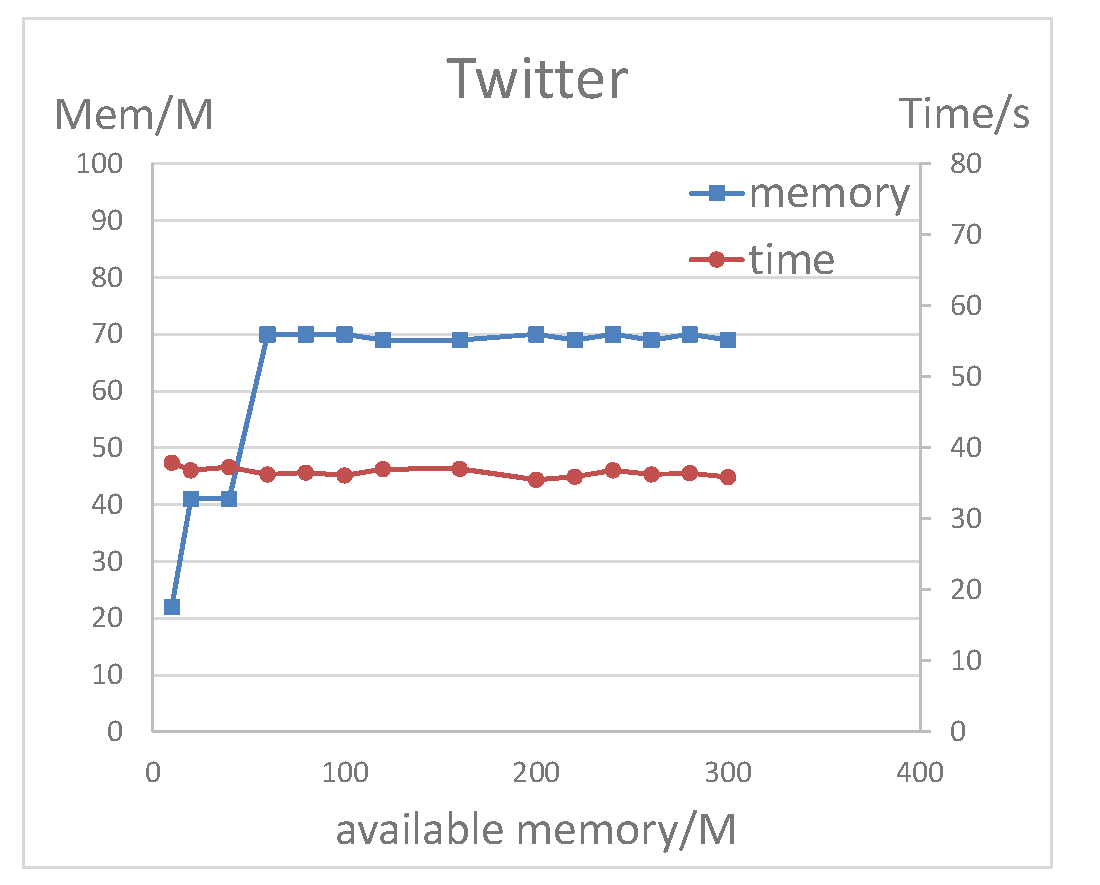
\includegraphics[width = 1.61in]{fig/twitterMemTime.eps}\label{fig:twitterMemTime}}\ \
    \hspace{0.5pt}
  \subfloat[Overall performance on web-BerkStan]{\includegraphics[width = 1.61in]{fig/webMemTime.eps}\label{fig:webMemTime}}\ \
   \hspace{0.5pt}
  \subfloat[Overall performance on Google]{\includegraphics[width = 1.61in]{fig/googleMemTime.eps}\label{fig:googleMemTime}}\ \
     \hspace{0.5pt}
  \subfloat[Overall performance on Pareto]{\includegraphics[width = 1.61in]{fig/paretoMemTime.eps}\label{fig:paretoMemTime}}\ \ 
    \caption{Overall performance on various data sets.}
  \label{fig:overallPerformance} 
\end{figure*}

\begin{figure*}[htbp]
    \centering
  \subfloat[Performance comparison on Twitter]{\includegraphics[width = 1.61in]{fig/twitterComparison.eps}\label{fig:twitterComparison}}\ \
    \hspace{0.5pt}
  \subfloat[Performance comparison on web-BerkStan]{\includegraphics[width = 1.61in]{fig/webComparison.eps}\label{fig:webComparison}}\ \
   \hspace{0.5pt}
  \subfloat[Performance comparison on Google]{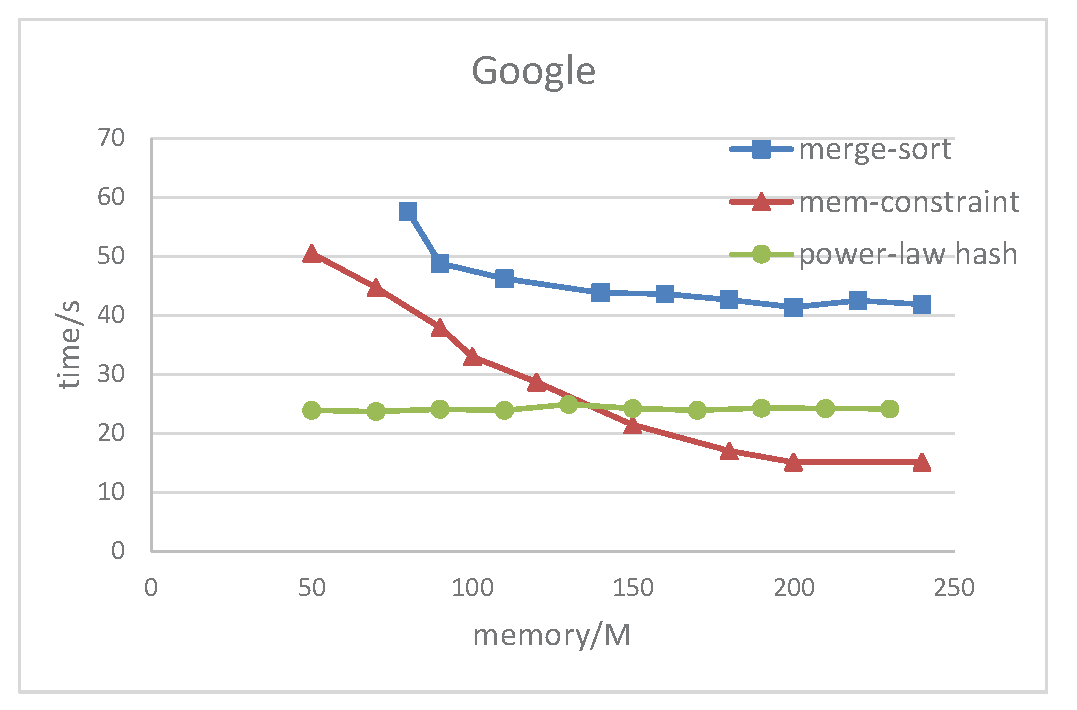
\includegraphics[width = 1.61in]{fig/googleComparison.eps}\label{fig:googleComparison}}\ \
     \hspace{0.5pt}
  \subfloat[Performance comparison on Pareto]{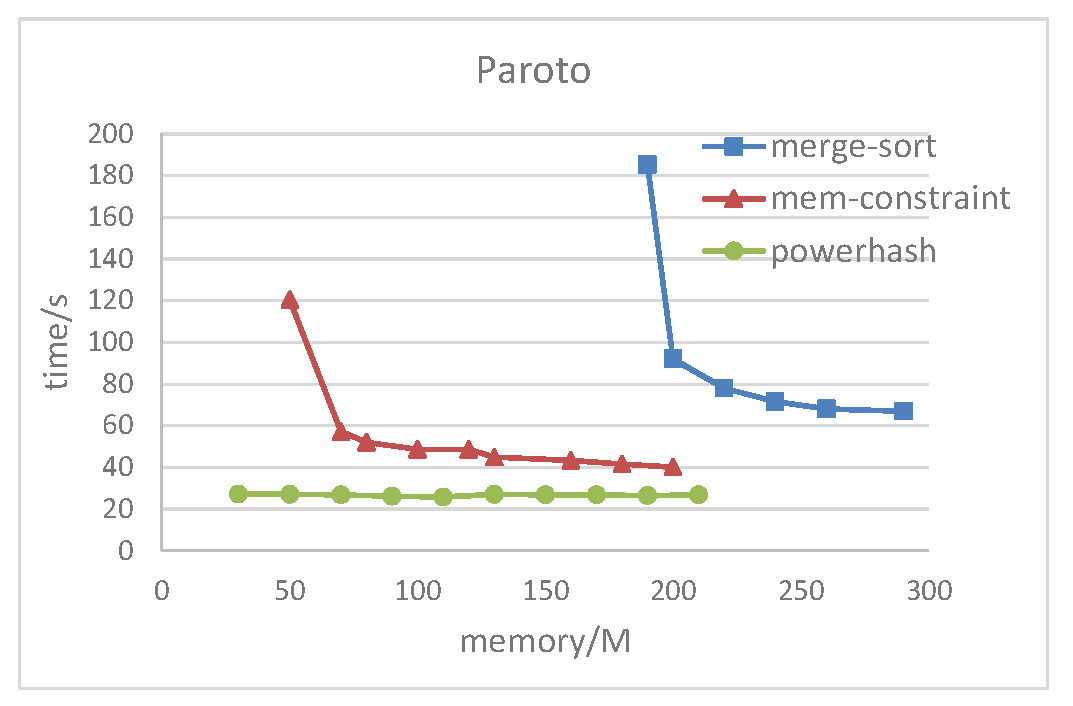
\includegraphics[width = 1.61in]{fig/paretoComparison.eps}\label{fig:paretoComparison}}\ \ 
    \caption{Performance comparison on various data sets.}
  \label{fig:performanceComparison} 
\end{figure*}

All serial methods were implemented in C++, and compiled with g++ version 4.8.4 in Linux. The experiments were executed on a machine with two quad-core Intel CPUs at 2.67GHz and 32GB RAM.



\subsection{Overall Performance Evaluation}

The following experiments exhibits the overall performance of power-law hash and its performance comparison against merge-sort and memory-constraint hash. When executing power-law hash algorithm on various data sets, the most important parameter --- the ratio of big groups in these data sets is set as 0.2 depending the Pareto principle, the expansion factor proposed in section \ref{sec:hash} to ensure each small group partition can be processed in memory safely is set as 2. 

Figure \ref{fig:overallPerformance} exhibits the overall performance of power-law hash for different data sets as showed in Table \ref{tab:dataset}, it shows the real memory consumption and grouping time with the available memory varying. We can see that power-law hash can complete the key grouping operation with a litle memory. As the available memory varies, the grouping time is almost unchanged, even if the available memory is very small, the time cost in which case is nearly equal to the time cost with sufficient memory (as shown in Figure \ref{fig:twitterMemTime} \ref{fig:webMemTime} \ref{fig:googleMemTime} \ref{fig:paretoMemTime}). The reason for this phenomenon is that the available memory only influences the partition of small groups if the ratio of big groups is fixed, the grouping time of big groups is the same in theory no matter how much memory is available, and the grouping time of small groups is also steady when the partition numbers are not much different, so the whole time cost of power-law hash is always keep stable. In addtion, the memory consumption grows stage by stage and then stays stable in Figure \ref{fig:overallPerformance}, each change of memory consumption represents a decrease of small groups partition number, the memory usage stays stable finally because there is enough memory to load the kv-pairs in small groups and the partition number decrease to 1. The minimal memory consumptions shown in Figure \ref{fig:overallPerformance} are the sizes of big group offset index, it is the low limit of available memory on various data sets.   

The next experiment investigates the scalability of our method. Figure \ref{fig:performanceComparison} shows the comparison of grouping time against merge-sort and memory-constraint hash with the memory available increasing, we list experimental results on different data sets. 
On the whole, our algorithm is almost distributed lower than other algorithms with limited memory in Figure \ref{fig:performanceComparison}, i.e., when the memory is not enough, our algorithm performs faster in the case of the same memory consumption, and it takes up less memory under the same time cost, the advantage is more obvious if the alailable memory is smaller, merge-sort algorithm is the slowest one among the three methods. For merge-sort and memory-constraint hash, the execution time continues to decline with the memory available increases constantly, when the memory is large enough to process kv-pairs in memory completely, the performance is no longer enhanced and grouping time stays stable, at that time memory-constraint hash degenerates into the pure hashing grouping method. The merge-sort needs 4 times memory and memory-constraint hash needs 2.5 times memory for Twitter to achieve the stable state compared to our algorithm as shown on Figure \ref{fig:twitterMemTime} \ref{fig:twitterComparison}, the experimental results on other data sets are similar with a little different multiples.

As shown in Figure \ref{fig:performanceComparison}, the grouping time of merge-sort is at least two times than power-law hash on these data set even if it achieves the steady state. When the available memory is not sufficient, the grouping time gap between the two method is larger . Compared to memory-constraint hash, the variance is greatest at the beginning of the line charts, the gap between their runtime continues to decline with the available increasing. When memory-constraint hash reaches the stable state, our algorithm achieves at least 25\% faster on web-BerkStan and at least 60\% faster on Pareto as shown in Figure \ref{fig:webComparison} \ref{fig:paretoComparison}. Memory-constraint hash can achieve the same performance on Twitter and Google, its time consumption is greater than power-law hash with the same memory before this point where they have the same runtime in Figure \ref{fig:twitterComparison} \ref{fig:googleComparison}, it can perform better than power-law hash on Google if the memory is sufficient. With the same time cost, the memory usage of our algorithm is smallest in most cases, because the power-law hash runtime almost keeps stable, it can reach the best state by the smallest memory compared to the other two approaches.
   
We make the following analysis to this phenomenon: recall to section \ref{sec:related}, for merge-sort algorithm, there is unnecessary computational overhead in aggregating kv-pairs, the sort process reduces its performance, its time cost is always highest even if the memory is enough. For memory-constraint hash, one or more buckets will be selected to spill to disk when the memory used has reached the threshold, these spilled partitions will be read back to re-aggregate subsequently. The power-law distributions makes it more difficult to divide the work data into small uniform portions. For a larger bucket spilled to disk, subsequent reading back and re-aggregating may lead to recursively execute the algorithm many times when the memory is limited, i.e., reading from and writing to the disk are more frequently, the I/O overhead increases sharply. However, power-law hash deals with the big groups and small groups separately, the big groups processed by indexing and filling, and the small groups are processed via partitioned hash grouping approach, the two grouping method used to process the big groups and small groups can be carried out with limited memory and avoid repeat access to disk as introduced in section \ref{sec:hash}, so the performance of memory-constraint hash is slower than power-law hash with the same limited memory. If there is enough memory, all kv-pairs can be loaded in memory, memory-constraint hash degenerate into the pure hashing grouping method, its performance will be faster than power-law hash as shown in Figure \ref{fig:googleComparison}. Therefore, our algorithm is able to more efficient in limited memory compared to other algorithms.

\subsection{Parameters Evaluation}
\begin{figure*}[htbp]
    \centering
  \subfloat[Ratio test on Twitter]{\includegraphics[width = 1.61in]{fig/twitterRatio.eps}\label{fig:twitterRatio}}\ \
    \hspace{0.5pt}
  \subfloat[Ratio test on web-BerkStan]{\includegraphics[width = 1.61in]{fig/webRatio.eps}\label{fig:webRatio}}\ \
   \hspace{0.5pt}
  \subfloat[Ratio test on Google]{\includegraphics[width = 1.61in]{fig/googleRatio.eps}\label{fig:googleRatio}}\ \
     \hspace{0.5pt}
  \subfloat[Ratio test on Pareto]{\includegraphics[width = 1.61in]{fig/paretoRatio.eps}\label{fig:paretoRatio}}\ \ 
    \caption{Ratio test on various data sets.}
  \label{fig:ratio} 
\end{figure*}
In the work, we also evaluate the impact on different parameters of power-law hash. We have experimentally evaluated on various data sets in Table \ref{tab:dataset} and theoretically analyzed the effects of these parameters on the algorithm. Figure \ref{fig:ratio} shows the strong scalability results for the algorithm.

\textbf{The ratio of big groups}. The ratio of big groups is the most important parameter in power-law hash, it determines the division between big groups and small groups. Compared with the real ratio of big groups in the data sets, a smaller ratio may lead to the unbalance of small group partitions because some big groups are judged as small groups, and then cause the redivision of small groups; a bigger ratio may result in a great offset index of big groups and then casues the waste of memory, so the selection of ratio is important. As shown in Figure \ref{fig:ratio}, the ratio is set from 0 to 1, the available memory is fixed and set as 50MB, power-law hash becomes the partitioned hash method when the ratio is 0, it turns to the indexing and filling method when the ratio is 1, their memory usage is much larger than 50MB in both cases and the out-of-memory problem will occur. With the ratio varying, the execution time decreases and then stays stable, the memory usage continues to decline and then continues to increase, the point with least memroy usage represents the offset index size and small group partition sizes are the most suitable, and the memory usage is under 50MB in this case, i.e., the algorithm can be executed in memory smoothly without out-of-memory problem. In Figure \ref{fig:webRatio} \ref{fig:googleRatio} \ref{fig:paretoRatio}, the memory usage is lowest when the ratio is 0.2, this phenomenon satisfies the Pareto principle. In Figure \ref{fig:twitterRatio}, our algorithm performs best when the ratio is 0.3. The experiment on these data sets can reflect the most appropriate ratio of big groups is the value around 0.2.
 
\textbf{The parameters of CM sketch}. The next experiment shows the effect of the CM sketch parameters. Recall from Distinguishing phase in section \ref{sec:hash} that the CM sketch are employed to reflect the distributions of group sizes, we sort a row of the CM sketch and then obtain the threshold between big group sizes and small group sizes according to the big groups ratio, then divide the big groups and small groups based on their rough sizes, so the width and depth of CM sketch can influence the judgement of big groups and small groups. According to the CM sketch introduction in section \ref{sec:related}: if the error of group sizes is within a factor of $ \varepsilon $ with probability $ \delta$, the depth is $\lceil ln(1/\delta)\rceil $, the width is $\lceil e/\varepsilon\rceil $, the depth can be set easily. The width of CM sketch determines the accuracy of threshold, it directly affects the division between big groups and small groups in Distinguishing phase. Figure 7 shows the memory usage and time cost on different data sets with the width varying.
\begin{figure}[htbp]
	\label{fig: CMPara}
    \subfloat[Runtime with different width]{\includegraphics[width = 1.68in]{fig/CMTime.eps}\label{fig:CMTime}}
       \hspace{0.23cm}
    \subfloat[Memory usage with different width]{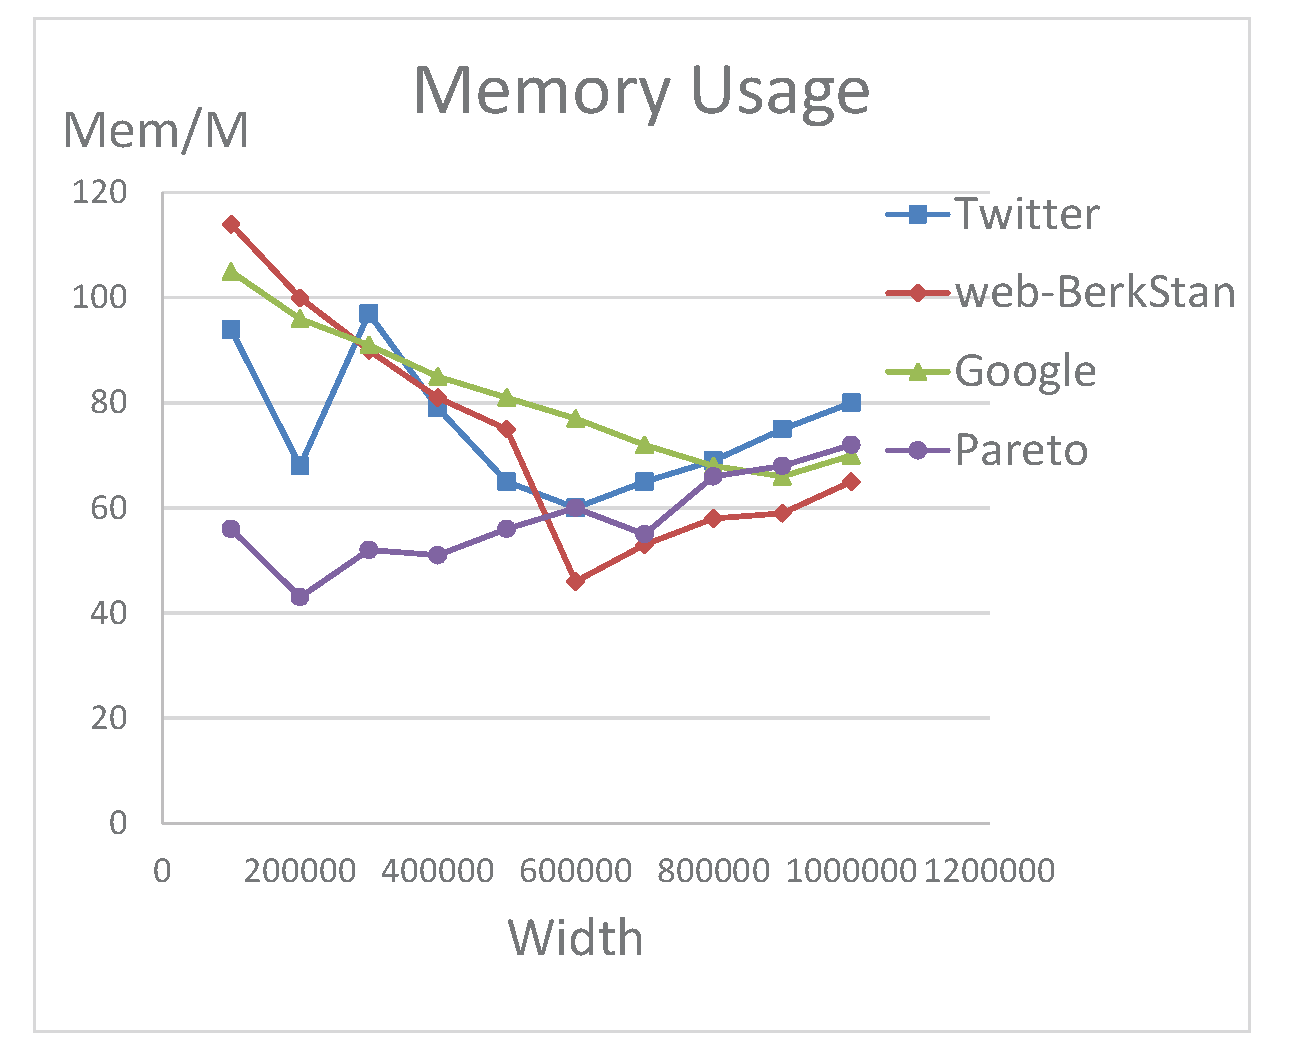
\includegraphics[width =1.68in]{fig/CMMem.eps}\label{fig:CMMem}}\\    
	\caption{Runtime and memroy usage with different width of the CM sketch.}	
	
\end{figure}

The runtime on each data set is almost steady as shown in Figure \ref{fig:CMTime}, the memory usage is influenced by the width of CM sketch as shown in Figure \ref{fig:CMMem}, it is appropriate to set the width from 400000 to 800000 with little memory waste.   

\subsection{Phase Evaluation}
In this subsection, we discuss the impact and interrelated factor on Distinguishing phase, Indexing and Filling phase, Partitioned hash phase. Figure \ref{fig: PhaseEvaluation} shows the time percentage and memory consumption on the three phases. 
%Distinguishing phase studies the global knowledge of group size information, Indexing and Filling phase generates an offset index that contains the output information of big groups and then groups the big groups by file random access on the basis of offset index. Partitioned hash phase deals with the small groups in memory and then append them to result file.
\begin{figure}[htbp]	
	\label{fig: PhaseEvaluation}
    \subfloat[Time percentage of each phase]{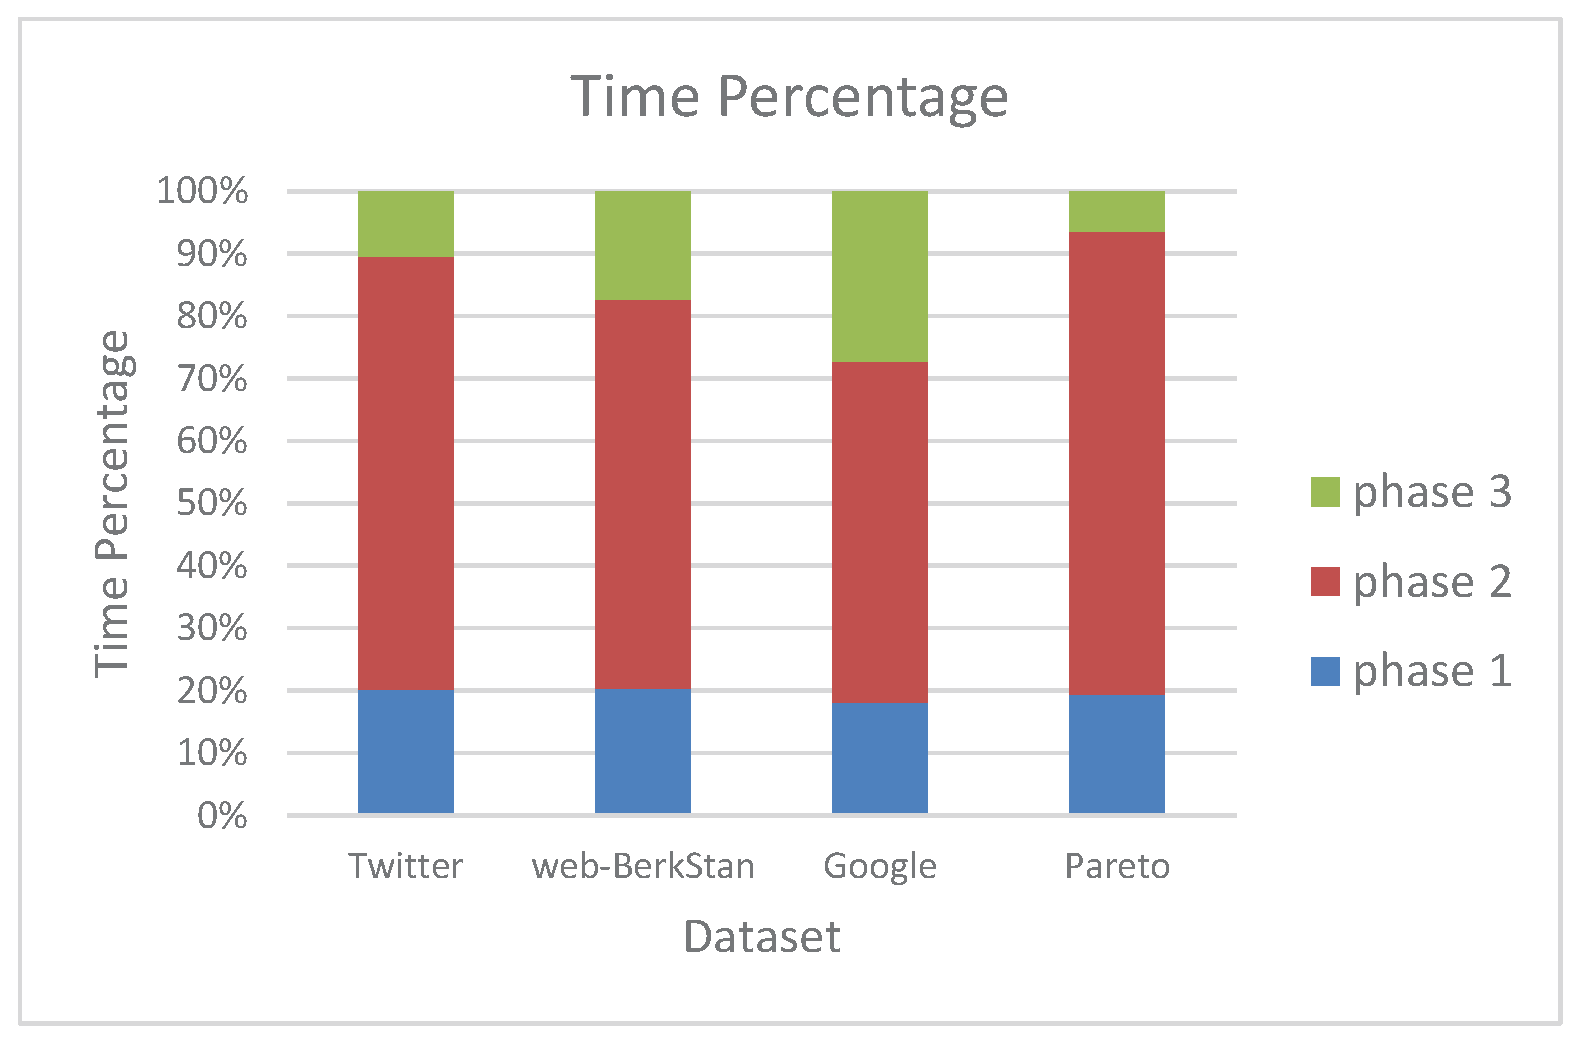
\includegraphics[width = 1.68in]{fig/TimePercentage.eps}\label{fig:TimePercentage}}
    \hspace{0.23cm}
    \subfloat[Memory usage of each phase]{\includegraphics[width =1.68in]{fig/MemPhase.eps}\label{fig:MemPhase}}\\    
	\caption{Runtime and memroy usage comparison between each phase.}
		
\end{figure}

Figure 8 shows the time percentage of the three phases on different data sets. We can notice that the time percentage of Distinguishing phase is close to 10\%, i.e., the preparation time of key grouping operation occupies 10\% of the total time. The Indexing and Filling for big groups take up most of the total time, the Partitioned hash phase groups the small groups with little time cost. This phenomenon satisfies expected result, the third phase is finished in memory so its time cost is small, the majority of the data set is processed in the second phase, and lots of time is spent on seek operations, so its time percentage is highest.

We also compare the memory usage for the three phases on various data sets as depicted in Figure \ref{fig:MemPhase}. The mark point on each line separates the three phases. The memory usage keep stable in phase 1, it reflects the size of CM sketch, then it increases over time gradually in phase 2, its growth represents the generation of offset index, it decreases after the memory occupied by the CM sketch being released. In the phase 3, the memory usage is also steady because the partition of small groups is balanced and each partition size is almost the same.



